\section{KFAC: approximating $\tilde{F}^{-1}$ as block-diagonal}
\frame{\tableofcontents[currentsection, hideothersubsections]}

\begin{frame}
\frametitle{KFAC: approximating $\tilde{F}^{-1}$ as block-diagonal}
Recall:
\begin{figure}
    \centering
    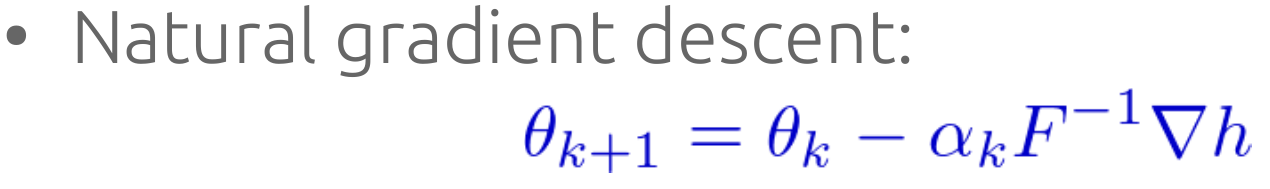
\includegraphics[scale=0.2]{natgrad}
\end{figure}

We already have $\tilde{F} \approx F$, then: \\
how to \textbf{efficiently} compute $\tilde{F}^{-1}$ or its product, $\tilde{F}^{-1}\nabla h$?
\end{frame}

\begin{frame}
\frametitle{KFAC: approximating $\tilde{F}^{-1}$ as block-diagonal}
Structure in the inverse Fisher:
\begin{figure}
    \centering
    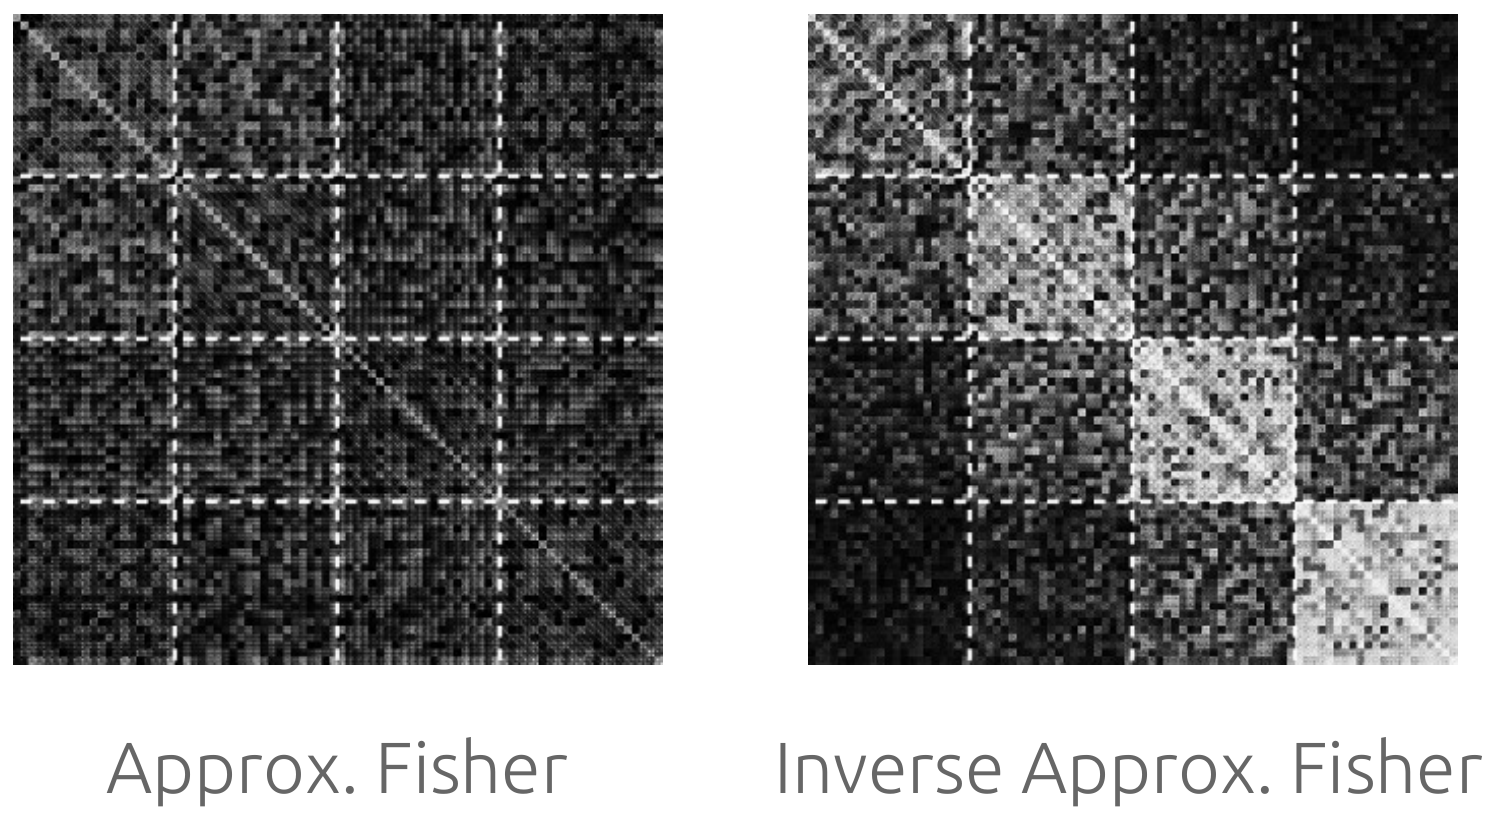
\includegraphics[scale=0.2]{kfac_06}
\end{figure}
(plotting absolute value of entries, dark means small)
\end{frame}

\begin{frame}
\frametitle{KFAC: approximating $\tilde{F}^{-1}$ as block-diagonal}
inverse of diagonal matrix
Structured inverses (Pourahmadi, 2011)

\end{frame}
